\documentclass{article}

% Packages
\usepackage{graphicx}
\usepackage{indentfirst}
\usepackage{hyperref}
\usepackage{hyperref} \hypersetup{
  colorlinks=true,
  linkcolor=black,
  citecolor=black,
  urlcolor=blue,
}
\usepackage{float}

\title{%
  CSCI 5481 Final Project \\
  \large Quantum machine learning in bioinformatics
}
\author{Brian Cooper \\ coope824@umn.edu \\ University of Minnesota}
\date{\today}

\begin{document}
\maketitle

\section{Abstract}
  Quantum computing is an emergent field that provides promising potential for the field of bioinformatics. Among various problems, classification is a common task in bioinformatics machine learning tasks for identifying and predicting classes of objects, such as organisms or genes. Using a quantum variant of the classical support vector machine, a quantum model can be created in a similar manner to a classical support vector machine model for making predictions. Applied quantum computing is quite new, and it is not commonly used in modern bioinformatics experiments. Here, it is demonstrated that quantum computing frameworks, although in their infancy, can be used to design and test classification models, and are robust enough to prototype. The accuracy of the quantum support vector machine is demonstrated to compare competitively with its classical counterpart, despite claims that quantum computing is not yet mature enough for widespread use. This challenges the current stigma associated with quantum computing. These results demonstrate that quantum computing may be ready for testing in modern experiments extending beyond bioinformatics into other scientific domains.

\section{Related Work}
  Quantum computing has a rich theoretical history, but not many have pursued it in an applied and experimental context. Biamonte, et al.~\cite{biamonte} argue that the foundation for quantum machine learning algorithms is strong, yet considerably limited by hardware and software challenges. They clarify that certain devices (such as annealing quantum computers) \textit{have} been built with apparently large qubit counts (2000, for example), although they do not communicate with each other well at such a scale yet, so there is ample room for improvement. An important point in~\cite{schuld} is that the ability to simulate the actual, concrete learning process in quantum systems is unsatisfactorily documented, and thus requires more development. They emphasize that we need to be careful in the wishful optimism of quantum computing's usefulness to machine learning -- especially considering its novelty. In contrast to these worldviews, both~\cite{biamonte} and~\cite{schuld} project that machine learning has a bright future when utilizing quantum processing power, and they mention that significant advancements have been made when it comes to hardware.

\section{Methods}
  Qiskit~\cite{ibm}, a Python quantum computing API and framework from IBM, was used to design the models and execute the classification tests. Qiskit provides two distinct methods for performing quantum computing experiments:

    \begin{itemize}
      \item{Running tasks on real quantum computing hardware (connected to IBM Q computers with an API)}
      \item{A built-in quantum hardware simulator for performing experiments on a classical computer}
    \end{itemize}

  The simulator was chosen, as I do not have any academic credit required to perform experiments on real quantum computing hardware. This necessarily rules out any accurate analysis of the time and space complexities, since quantum computing mathematics is calculated within a classical computer environment. Quantum computing algorithms are, of course, designed to be run on quantum hardware, so the computational time and space cannot be accurately gauged in this manner. Qiskit does provide GPU acceleration support through its QCGPU communication package~\cite{qcgpu}. \\

  Multivariate data was selected from the UCI Machine Learning Repository~\cite{uci}. Instances from three datasets were used:

    \begin{itemize}
      \item E. Coli~\cite{ecoli}
      \item Yeast~\cite{yeast}
      \item Mice Protein Expression~\cite{mouse}
    \end{itemize}

  The full E. Coli (336 instances, 7 features) and yeast (1484 instances, 8 features) datasets were used, but only a subset of the mouse dataset was used (553 instances -- after removing instances with missing attributes -- and the first 9 features). This is because the original size of the mouse dataset, with 1080 instances and 82 features, would be intractable for a classical quantum simulation without distributing the task with GPU acceleration or a real quantum computer. \\

  A support vector machine with a radial-basis kernel was chosen (same kernel for both types of support vector machines -- classical and quantum). Each of the datasets was split into 70\% testing data and 30\% training data. Principal component analysis (PCA) dimensionality reduction was used to reduce the space to two dimensions, which matches the number of qubits used in the quantum support vector machine. The data space, after dimensionality reduction, can be visualized in Figure \ref{fig:data}.

  \begin{figure}[h]
    \centering
    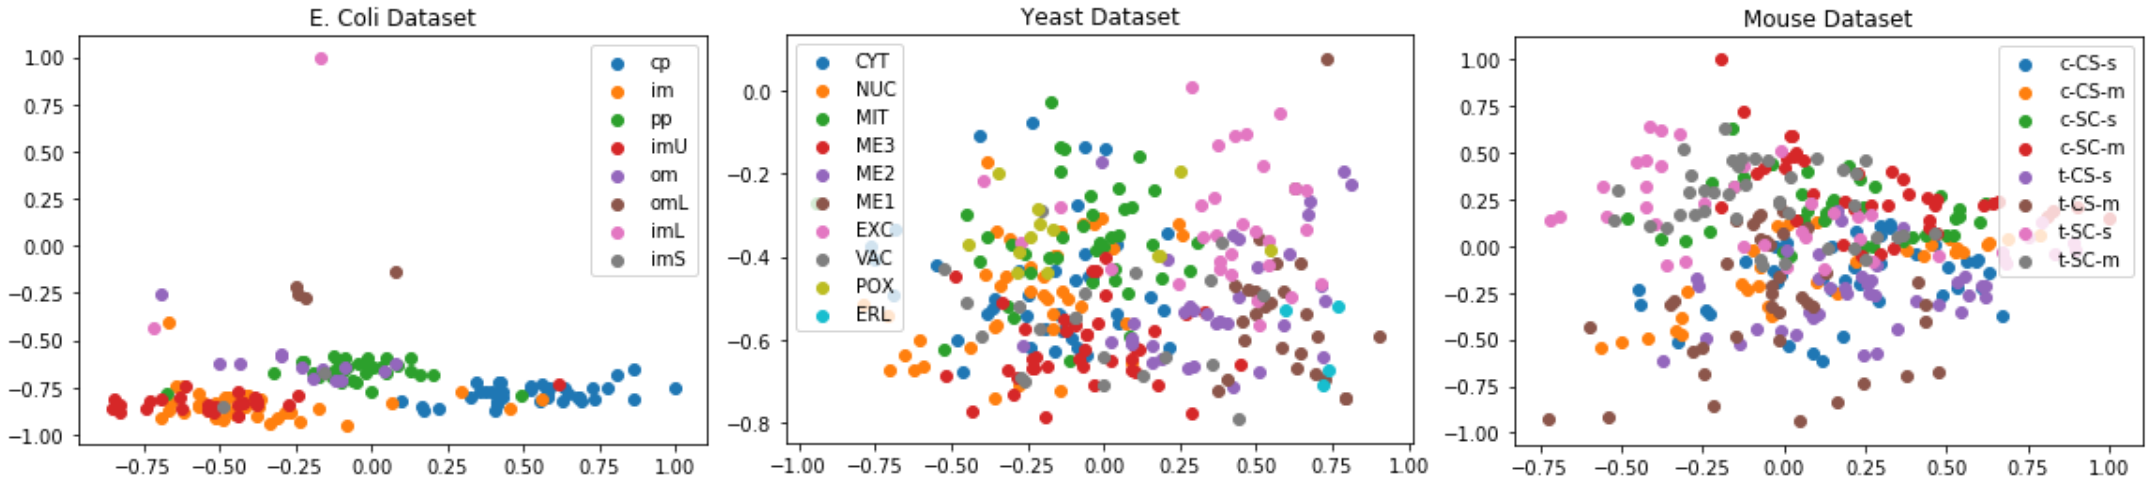
\includegraphics[width=1\textwidth]{data.png}
    \caption{\label{fig:data}Visualization of the data.}
  \end{figure}

\section{Results}
  Table \ref{table:accuracy} shows the accuracy results of the classical and quantum support vector machine experiments on all three datasets. Figure \ref{fig:results} shows the same results visually. \\

  \begin{table}[h]
    \centering
    \begin{tabular}{c|c|c|}
    \cline{2-3}
                                  & Classical SVM & Quantum SVM \\ \hline
    \multicolumn{1}{|c|}{E. Coli} & 90\%          & 70\%        \\ \hline
    \multicolumn{1}{|c|}{Yeast}   & 45\%          & 49\%        \\ \hline
    \multicolumn{1}{|c|}{Mouse}   & 43\%          & 22\%        \\ \hline
    \end{tabular}
    \caption{\label{table:accuracy}Model accuracy results.}
  \end{table}

  \hfill \break

  \begin{figure}[h]
    \centering
    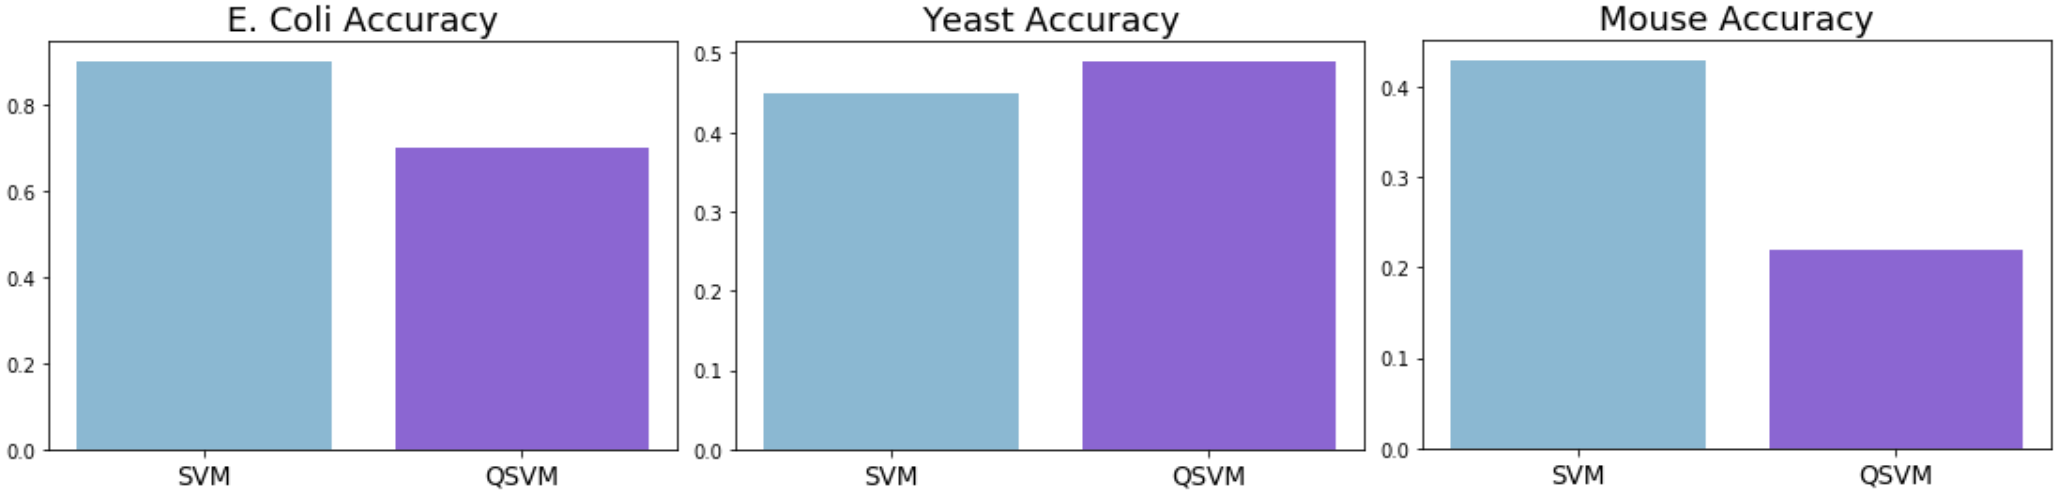
\includegraphics[width=1\textwidth]{accuracy.png}
    \caption{\label{fig:results}Visual model accuracy results.}
  \end{figure}

  The quantum implementation of SVM created a model with slightly better accuracy on the yeast dataset (49\% vs. 45\%). However, it did not perform as well on the E. Coli (70\% vs. 90\%) and mouse datasets (22\% vs. 43\%). For a deeper analysis, it would be ideal to perform other quantum machine learning classification algorithms (or different kernels) on the data to provide more benchmarks. Precision, recall, and F1-score are some measures that could be used to further analyze the experimental output. \\

  The relatively lower accuracy on the mouse dataset may be improved by using more data from the mouse dataset (up to the entire set), which would be more practical with real quantum hardware due to its scale, as described previously in the \textit{Methods} section. Although the removal of data results in lower accuracy, the primary focus of this research is to compare the performance of the two support vector machine approaches, rather than focus on optimizing the model performance itself. \\

  A parameter that can be specified when constructing an algorithm in Qiskit is the number of shots, which specifies how many times a quantum circuit is repeated. The reason it's desirable to repeat the circuit multiple times is to gradually build up distribution statistics of the logical circuit results. In Qiskit, this number is 1024 by default. The value was reduced to 256 to speed up the computation time. Even when reducing the number of shots to 256, the quantum algorithms still took a very long time compared to the classical approach. Overall, each of the three quantum algorithm runs (with all 256 shots included) took several hours, while performing the same task classically completed in under a minute. Assuming the QASM simulator is accurate and factors in noise and other environmental factors, using a physical IBM Q backend should produce similar results to those above with faster speed.

\section{Conclusion}
  This work challenges the notion that quantum computing algorithms are not practical for modern use. The hardware is indeed limited, however, Qiskit and other frameworks enable convenient quantum algorithm usage and lower the barrier for entry by opening the source code to the public. \\

  Overall, the quantum computing space may be something to consider for future scientific work. Quantum computers will supposedly be excellent at solving optimization problems, which are at the core of artificial intelligence and machine learning problems. Thus, it is likely that bioinformatics will enjoy a surge of innovation as quantum computers establish their place in society.

\newpage
\bibliographystyle{plain}
\raggedright
\bibliography{./final-project}

\end{document}
